%!TEX TS-program = pdflatexmk

% Copyright (c) 2018 - 2022, Martin Scheidt (ISC license)
% Permission to use, copy, modify, and/or distribute this file for any purpose with or without fee is hereby granted, provided that the above copyright notice and this permission notice appear in all copies.

\documentclass[border=2]{standalone}

\usepackage[dev]{tikz-trackschematic}

\begin{document}
  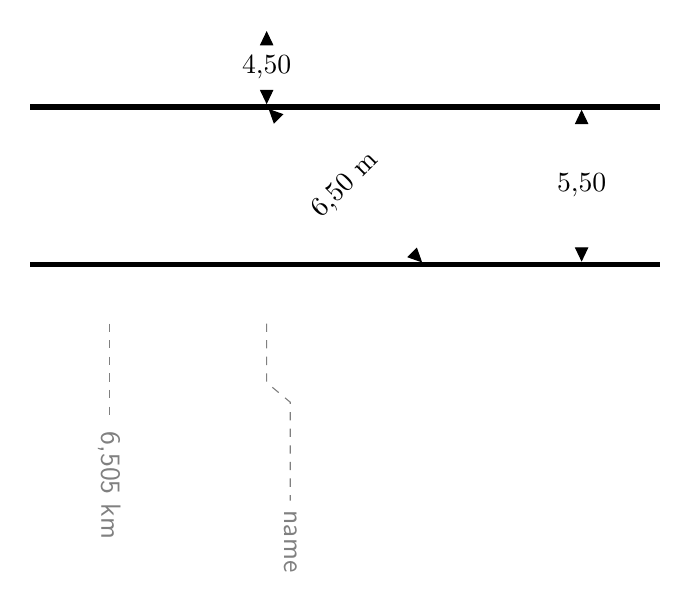
\begin{tikzpicture}
  
    \foreach \i in {1,2,3}{% base coordinate
      \coordinate (A\i) at ($(0,0) + 2*(0,-\i)$);% base coordinate
      \coordinate (B\i) at ($(8,0) + 2*(0,-\i)$);% base coordinate
    }

    \foreach \i in {1,2}{% draw main tracks on base coordinate
      \maintrack (A\i) --   (B\i);
    }

    \foreach \i in {1,2}{% coordinates for testing symbols
      \coordinate (X\i-1) at ($(1,0) + 2*(0,-\i)$);
      \coordinate (X\i-2) at ($(3,0) + 2*(0,-\i)$);
      \coordinate (X\i-3) at ($(5,0) + 2*(0,-\i)$);
      \coordinate (X\i-4) at ($(7,0) + 2*(0,-\i)$);
    }

    \trackdistance between (3,-1) and (X1-2) label (4,50);
    \trackdistance between (X1-2) and (X2-3) label (6,50~m);
    \trackdistance between (X1-4) and (X2-4) label (5,50);

    \tikzset{hectometer base={(A3)},orientation=right};
    \hectometer[] at (X2-1) mileage (6,505~km);
    \hectometer[shift label={(0.3,-1)}] at (X2-2) mileage (name);
    % \measureline between (a) and (b);

  \end{tikzpicture}
\end{document}